%!TEX root = ../../thesis.tex



\subsection{Exoplanets to low mass stars}

Exoplanetary detections have challenged the theoretical formation models with their variety and distribution of sizes, locations For instance, the discovery of the hot-Jupiter class (large mass planets on close in orbits) challenged the accepted planet formation theories at the time~\citep[.e.g][]{pollack_formation_1996} in which our Solar System was thought to be typical with small rocky planets close to the Sun and large giant planets further away.

The characterizatio of exoplanets with the detection of exoplanetary atmospheres allows for the constraints of exoplanetary composition and formation mechanisms.

For rocky planets models there are infinite combinations of Mass-radius. Models of the mass and radius for Earth like rocky planets for different compositions are given in \fref{fig:mass_radius_relation_composition} with some Solar System planets and two exoplanets shown. The composition varies from solid iron core (red)) through a combination of silicates \textbf{(rocks)} out to 100\% water (blue).


For planets with atmospheres, especially gas giants on close in orbits, the mass radius relation is more complicated with inflation due to atmospheric heating. 



There are two main fomation mechanisms , core accretion and disk instability. The presence of all the hot jupiters is due to Migration in which the planets trade angular mmentum with the planet forming disk to change postion.

As the mass of the companion increases 
Brown dwarfs

Several authors have found there are correlations with stellar metallicity, but less so with rocky planets.


- Small densities - mercury like  density~\citet{dittmann_temperate_2017, santerne_earthsized_2018, ment_second_2018} rocky super-earths\todo{move elsewhere}\\


\subsection{Exoplanet distribution} 4 different groups

\fref{}


\begin{figure}
    \centering
    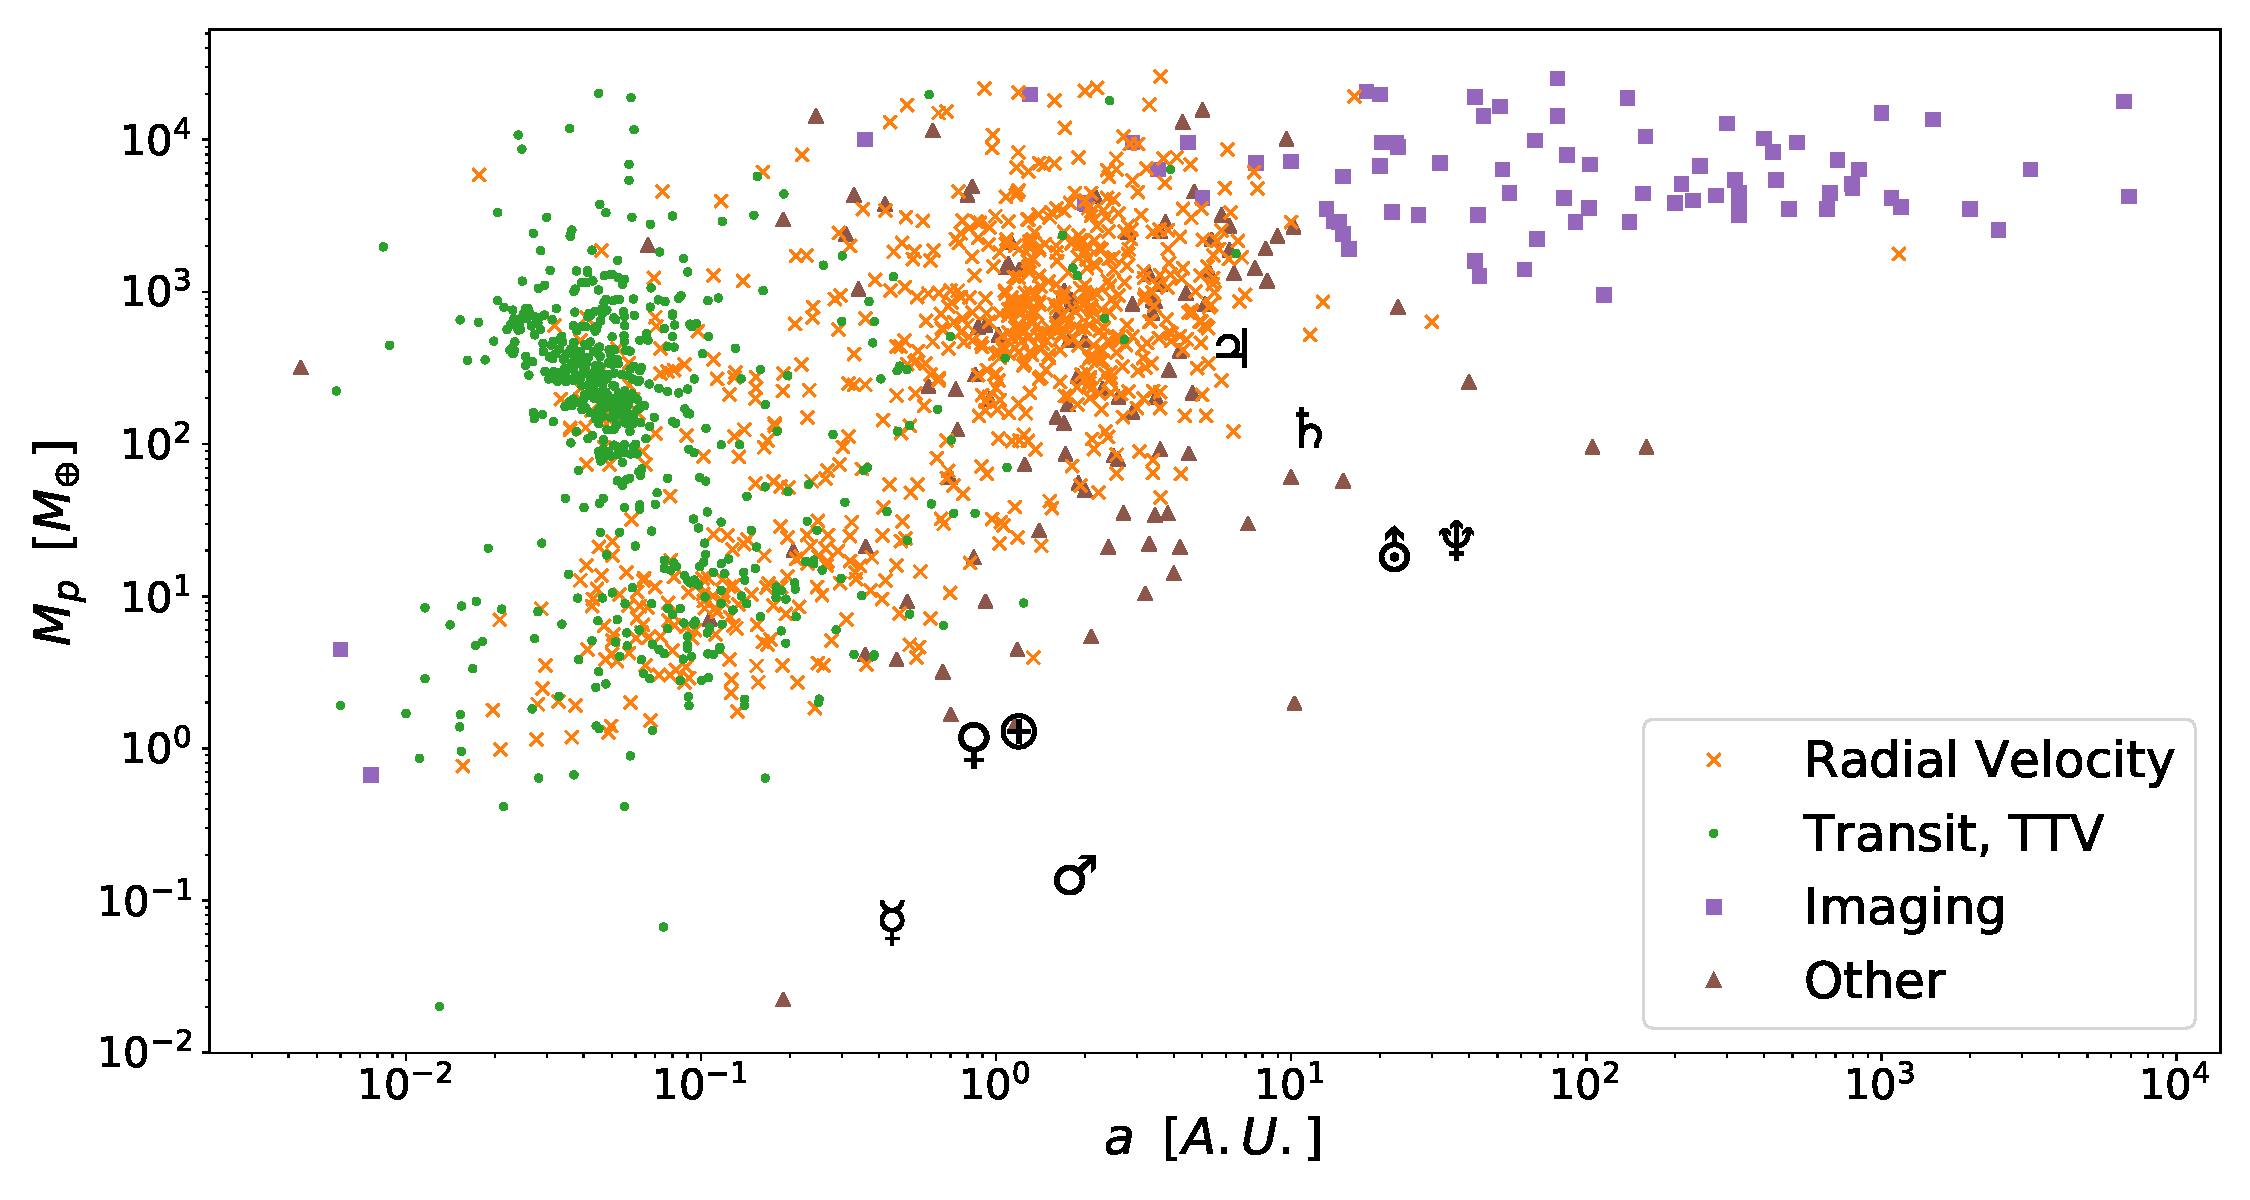
\includegraphics[width=0.\linewidth]{./figures/introduction/exoplanetEU_a_mass.pdf}
    \caption{Distance mass diagram.
        The symbols indicate the location of the solar system planets, $\mercury$-Mercury, $\venus$-Venus, $\earth$-Earth, $\mars$-Mars, $\jupiter$-Jupiter, $\saturn$-Saturn, $\uranus$-Uranus, $\neptune$-Neptune. Data from \href{http://ww.exoplanet.eu}{exoplanet.eu} October 2018}
    \label{fig:pltoverlayadd}
\end{figure}


Explore what these method have found with exoplanet populations.


\begin{figure}[t]
    \centering
    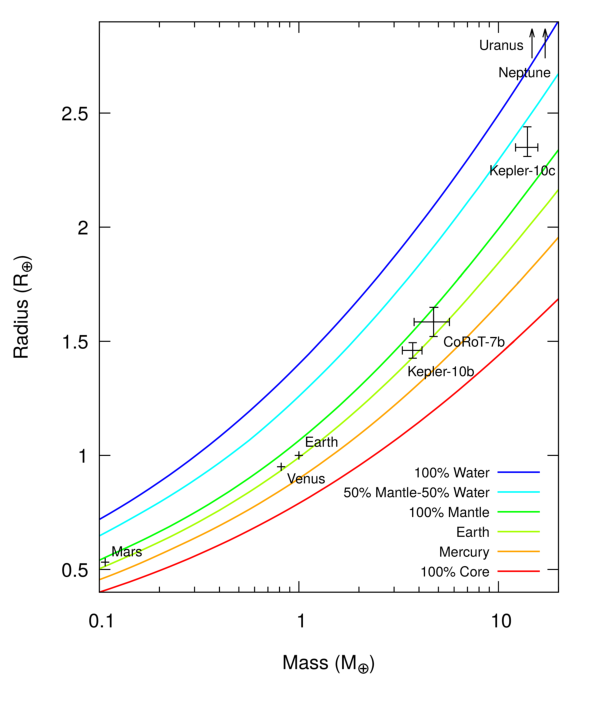
\includegraphics[width=0.4\linewidth]{./figures/introduction/Mass_radius_relation-compostion_Brugger_2017.pdf}\\
    \caption{Mass-Radius relationship for (super) Earth-like planets with composition contours. Adapted from~\citet{brugger_constraints_2017}}
    \label{fig:mass_radius_relation_composition}
\end{figure}

MR relation ship image arXiv:1506.05097~\citet{chen_probabilistic_2016}

\begin{figure}[t]
    \centering
    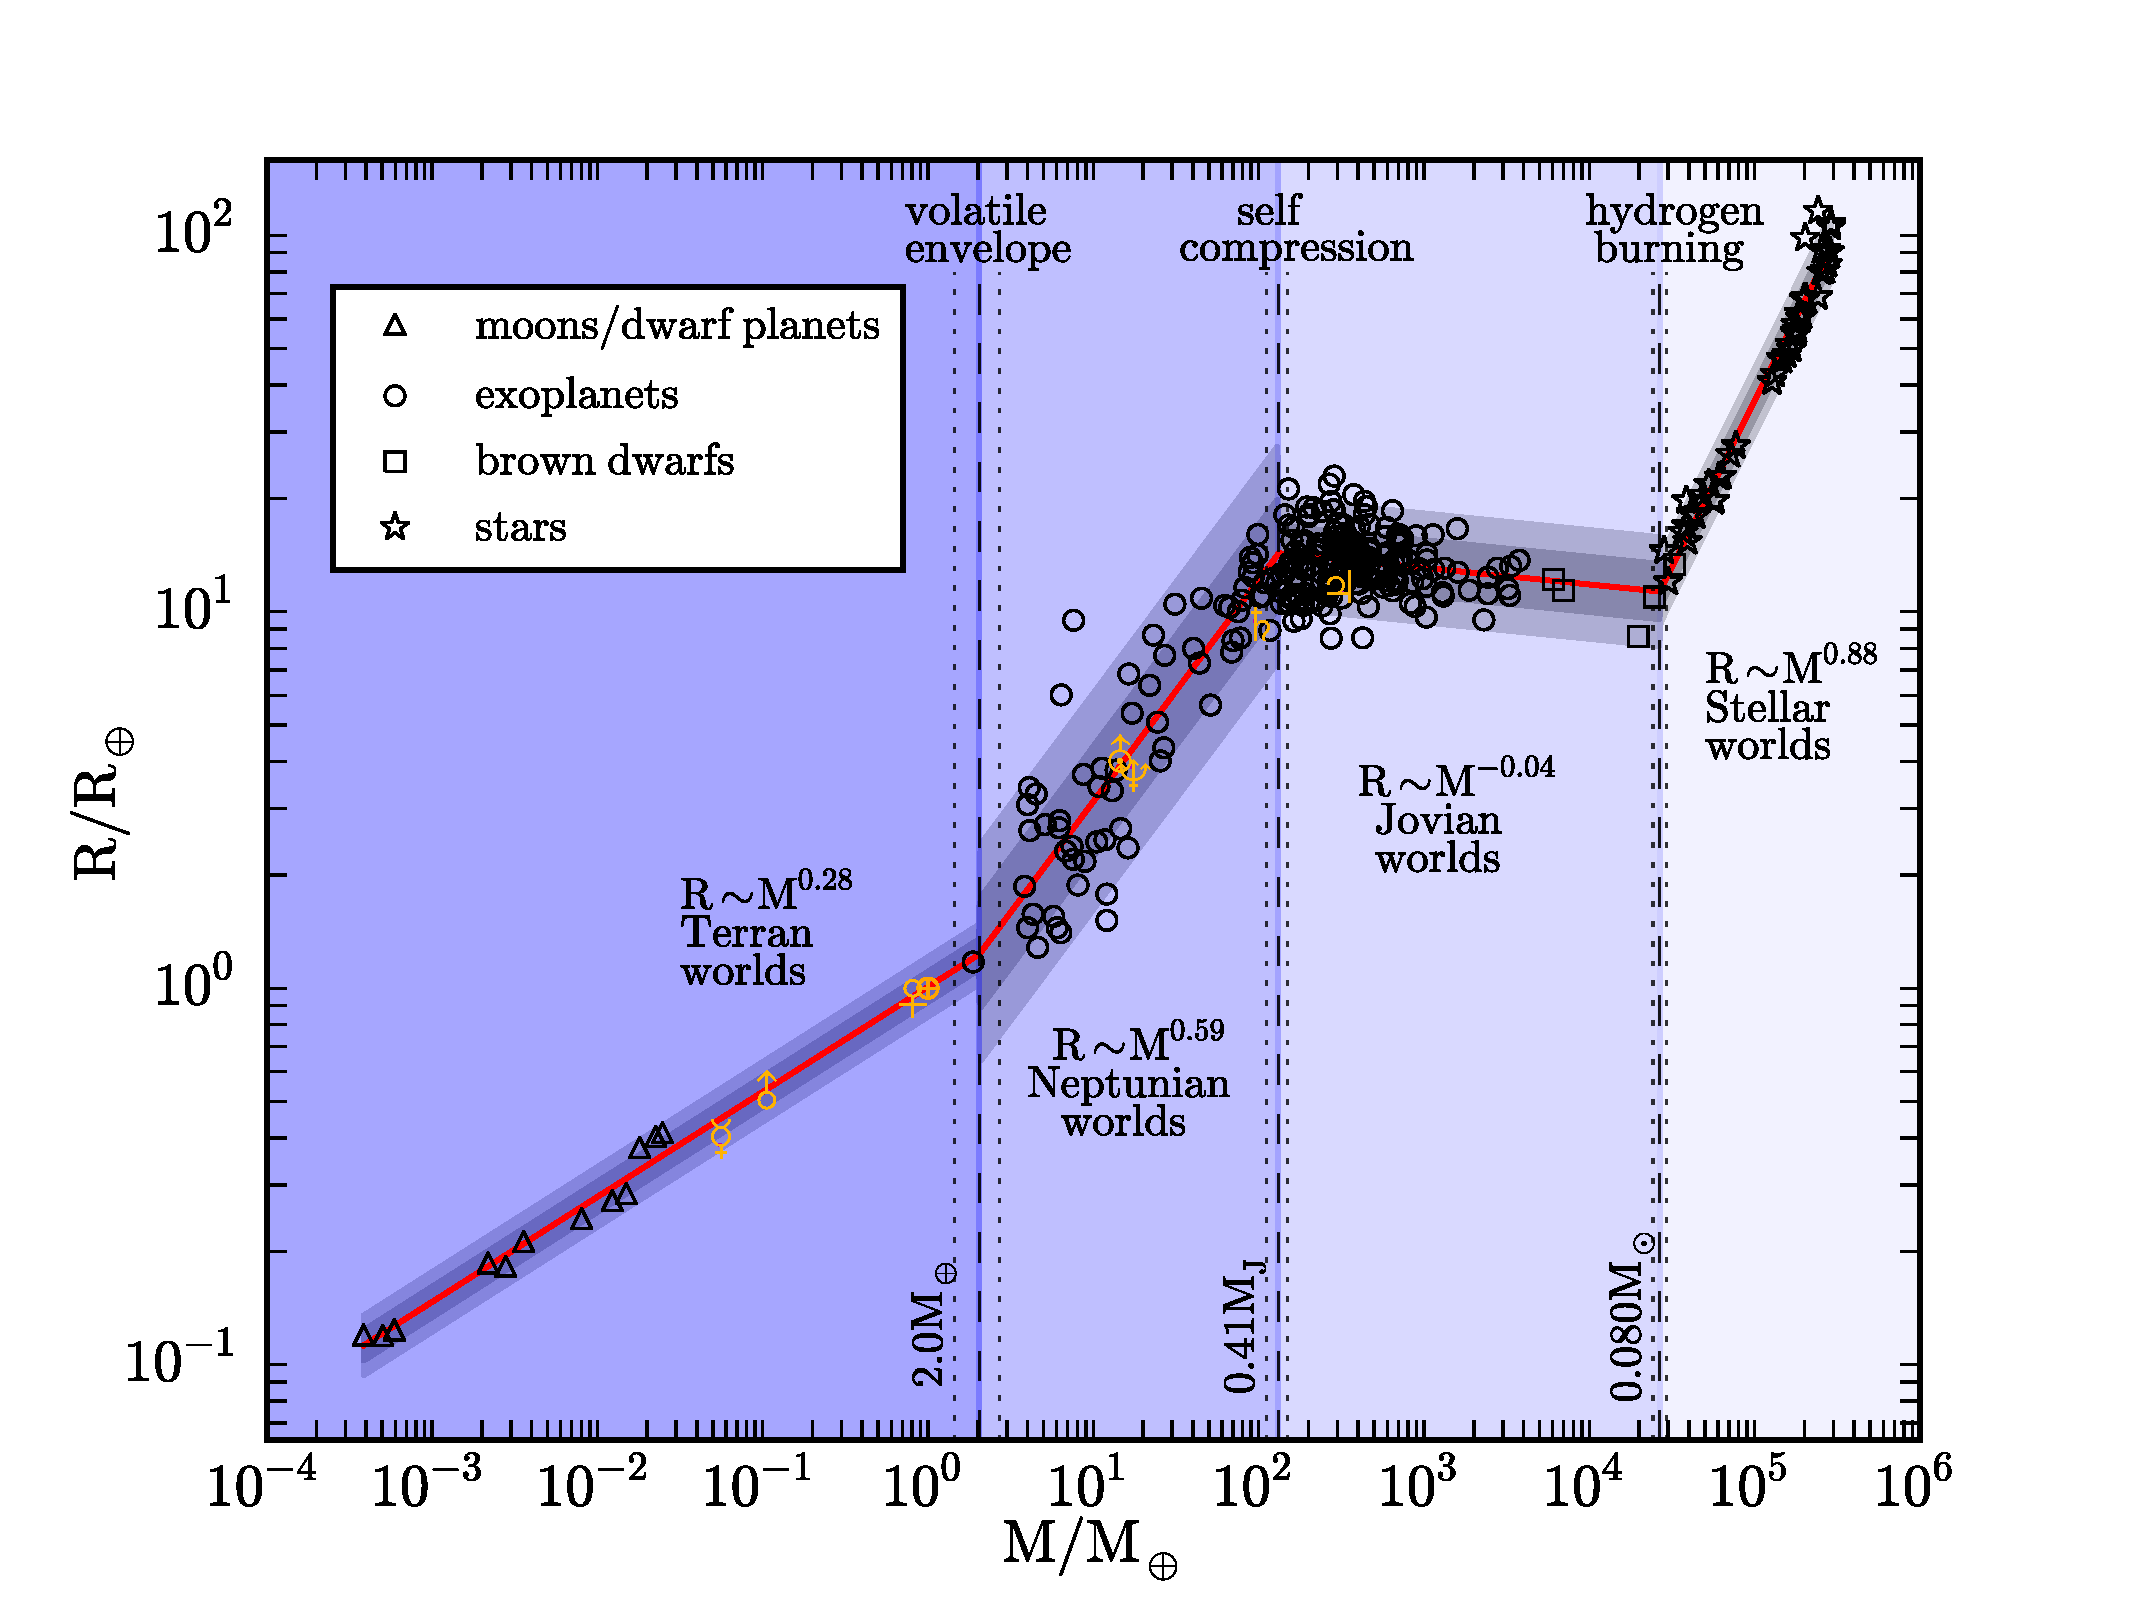
\includegraphics[width=0.9\linewidth]{./figures/introduction/mass_radius_relation.pdf}  \\
    \caption{Left: Mass-Radius relationship from planets to stars~\citet{chen_probabilistic_2016}.}
    \label{fig:mass_radius_relation}
\end{figure}


\citep{santos_observational_2017} Santos et al 2017 \todo{read and quote}  Observational evidence for two distinct giant planet populations
 

double peak histogram from an {RV} paper?? Faria 2018?


did they form from the molecular cloud when the star was forming or from the remnants of the disk after the star formed like exoplanets....?


Theory of migration in the disk through  angular moment transfer (cite).


\section{Conditions for life?}
habitable zone stuff
proxima b
Jorges paragraph....
